\documentclass[25pt, a0paper, portrait, blockverticalspace=.5cm]{tikzposter}
\usepackage[utf8]{inputenc}
%\usepackage{amssymb}
%\usepackage{amsfonts}
%\usepackage{amsmath}
%\usepackage{mathtext}
%\usepackage{mathtools}
\usepackage{xfrac}
%\usepackage{enumitem}
\usepackage{makecell}
\usepackage{physics}

\let\vec\oldvec
\newcommand{\vec}[1]{\boldsymbol{#1}}

\usetheme{Simple}
\usecolorstyle{Russia}
\colorlet{blocktitlefgcolor}{black}

\usepackage{caption}
\captionsetup{font=large}
\usepackage{multicol}
\setlength\columnsep{0cm}

\title{\parbox{\linewidth}
	{\centering
		ELECTROSTATIC DEFLECTOR NUCLOTRON\\ MODERNIZATION FOR EDM EXPERIMENT	
}}

\author{\LARGE{S. Kolokolchikov\textsuperscript{1,2}, Y. Senichev\textsuperscript{1,2}, A. Aksentyev\textsuperscript{1,2,3}, A. Melnikov\textsuperscript{1,2,4},\\ P. Palamarchuka\textsuperscript{1,3}, E. Syresin\textsuperscript{5}, V. Ladygin\textsuperscript{5} \\
		\textsuperscript{1}Institute for Nuclear Research of the Russian Academy of Sciences, Moscow, Russia\\
		\textsuperscript{2}Moscow Institute of Physics and Technology, Dolgoprudny, Russia\\
		\textsuperscript{3}National Research Nuclear University MEPhI, Moscow, Russia\\
		\textsuperscript{4}Landau Institute for Theoretical Physics, Chernogolovka, Russia\\
		\textsuperscript{5}Joint Institute for Nuclear Research, Dubna, Russia}}

\begin{document}
\maketitle
\begin{columns}
\column{.33}

\block{INTRODUCTION}{\hfill

\par Considered the current Nuclotron structure for precision EDM-experiments as an independent synchrotron storage ring equipped with electrostatic deflectors. In this regard, the design must ensure the preservation and precise regulation of spin dynamics stability. Moreover, the initial purpose of the structure as a booster of polarized beams in the collider has been preserved.
}

\block{QUASI-FROZEN SPIN}{\hfill

\par For an ensemble of particles, the spin can be described as a classical vector and its dynamics in external electromagnetic fields is described by T-BMT equation [1]

\begin{equation}\label{eq:T-BMT}
\begin{aligned}
\dv{{\vec{S}}}{t} =&\left(\vec{\Omega}_{\text{MDM}}+\vec{\Omega}_{\text{EDM}}\right) \times \vec{S}, \\
\vec{\Omega}_{\text{MDM}}=&-\frac{q}{m \gamma}\left\{(\gamma G+1)\vec{B}_{\perp}+(G+1)\vec{B}_{\parallel}-\right. \\
&\left.-\left(\gamma G+\frac{\gamma}{\gamma+1}\right) \frac{\vec{\beta} \times \vec{E}}{c}\right\}, \\
\vec{\Omega}_{\text{EDM}}=&-\frac{q \eta}{2 m}\left(\vec{\beta} \times \vec{B}+\frac{\vec{E}}{c}-\frac{\gamma}{\gamma+1}\frac{\vec{\beta}}{c}\left(\vec{\beta}\cdot\vec{E}\right)\right).
\end{aligned} 
\end{equation}

	\par For EDM measurements, it is first necessary to compensate for MDM-effect. For this reason can be considered frozen spin method [2], involves an all-electric storage ring at "magic" energy for protons.
	\par An alternative approach is the quasi-frozen spin concept, based on the principle of sequential spin compensation [3].

\section*{Relative spin motion at QFS}  

	\par It is essential to ensure first condition that the orbital trajectory remains unperturbed, maintaining a closed orbit
	
	\begin{equation}
		\Phi_p^{\textrm{arc}}+\Phi_{p}^{\textrm{comp}}=\frac{2\pi}{N}\ \ \
		\label{eq:QFS_orbital}
	\end{equation}
	
	\par The second condition is to compensate MDM spin rotation in one period of the ring 
	
	\begin{equation}
		\Phi_s^{\textrm{arc}}+\Phi_{s}^{\textrm{comp}}=0,
		\label{eq:QFS_spin}
	\end{equation}
	
	\par Finally, can be received for rotation via magnetic or electric field in spin compensator element
	
	\begin{equation}
		\Phi_{p\mathrm{E}}^{\textrm{comp}} = - \Phi_{p\mathrm{B}}^{\textrm{comp}} = {\Phi}_{p}^{\text{arc}}\frac{\gamma^2 G}{G+1} =\frac{2\pi}{N}\frac{\gamma^2 G}{G+1}.
		\label{eq:deflection}
	\end{equation}
	
	\noindent No mention was made of the physical structure of the compensation element, only of the integral features of field components.

\section*{Spin compensation element length}

	The limitation on the strength of the electric field is much more significant than in the case of a magnetic field. Can be received the length of compensator element per one period
	
	\begin{equation}
		\begin{aligned}
			L_{\text{min}} = \Phi_{p\mathrm{E}}^{\text{comp}}R_{\mathrm{E}} & = 
			\frac{2\pi}{N}\frac{\gamma^2 G}{G+1}\frac{\kappa}{\mathrm{E}_{\text{max}}} = \\
			& = \frac{2\pi}{N}\frac{G}{G+1}\frac{mc^2}{e}\frac{\gamma(\gamma^2-1)}{\mathrm{E}_{\text{max}}}
			\label{eq:length_min}
		\end{aligned}
	\end{equation}
	
	\par For total length $L=L_{\text{min}}^{\text{total}} = N\cdot L_{\text{min}}$ and is independent from number of periods. Maximum attainable electric field are 10-13 MV/m [4], this corresponds to a magnetic field of the order of 70-90 mT accordingly, it will be used later for evaluation.

}

\column{.66}

\block{ELECTROSTATIC DEFLECTOR}{
		\begin{minipage}{0.47\linewidth}
			\centering deuteron case
			\begin{tikzpicture}
				\node (cone) at (0,0) {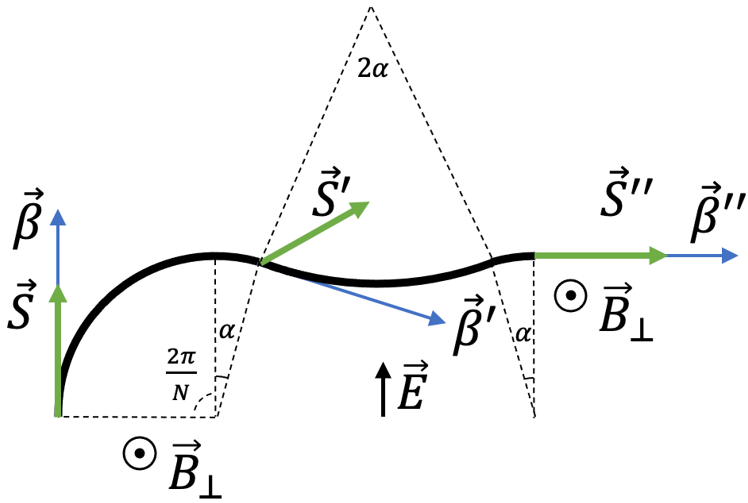
\includegraphics[width=\linewidth]{TEXPaper/img/TUPS031_f1}};
			\end{tikzpicture}
			proton case
			\begin{tikzpicture}
				\node (cone) at (0,0) {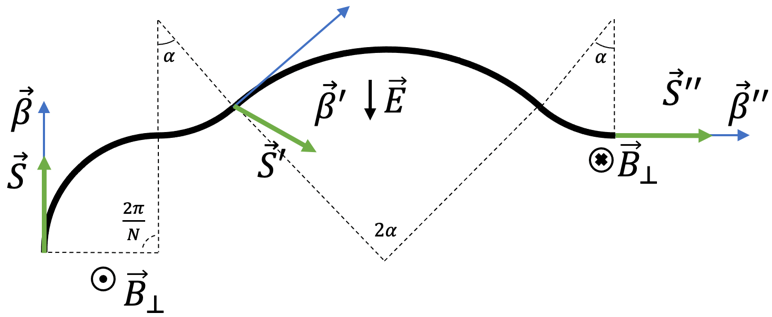
\includegraphics[width=\linewidth]{TEXPaper/img/TUPS031_f2}};
			\end{tikzpicture}
		\end{minipage}
		\hfill
		\begin{minipage}{0.45\linewidth}
			\par Pure electrostatic deflector designed to manipulate particle trajectories and spin dynamics by creating a radial electric field with non-zero curvature. This setup is particularly useful for creating bypass sections in addition to native straight sections, allowing for flexible experimental configurations. But it requires the usage of kicker magnet to deflect beam at bypass section.
			\newline
			\par For EDM measurements the energy determines by polarimeter needs as 270 MeV [5]. The mass-to-charge ratio of deuterons two times more than for protons. The anomalous magnetic moments are notably different: $G_{\text{p}} = 1.79$ and $G_{\text{d}} = -0.14$. The sign of rotation differs, this shows the necessity of rotating it by $\pi$ along the longitudinal axis. Additionally, the minimal achievable spin compensator length is longer for protons.
		\end{minipage}
		
		\begin{minipage}{0.3\linewidth}
			\begin{tikzpicture}
			\node (cone) at (0,0) {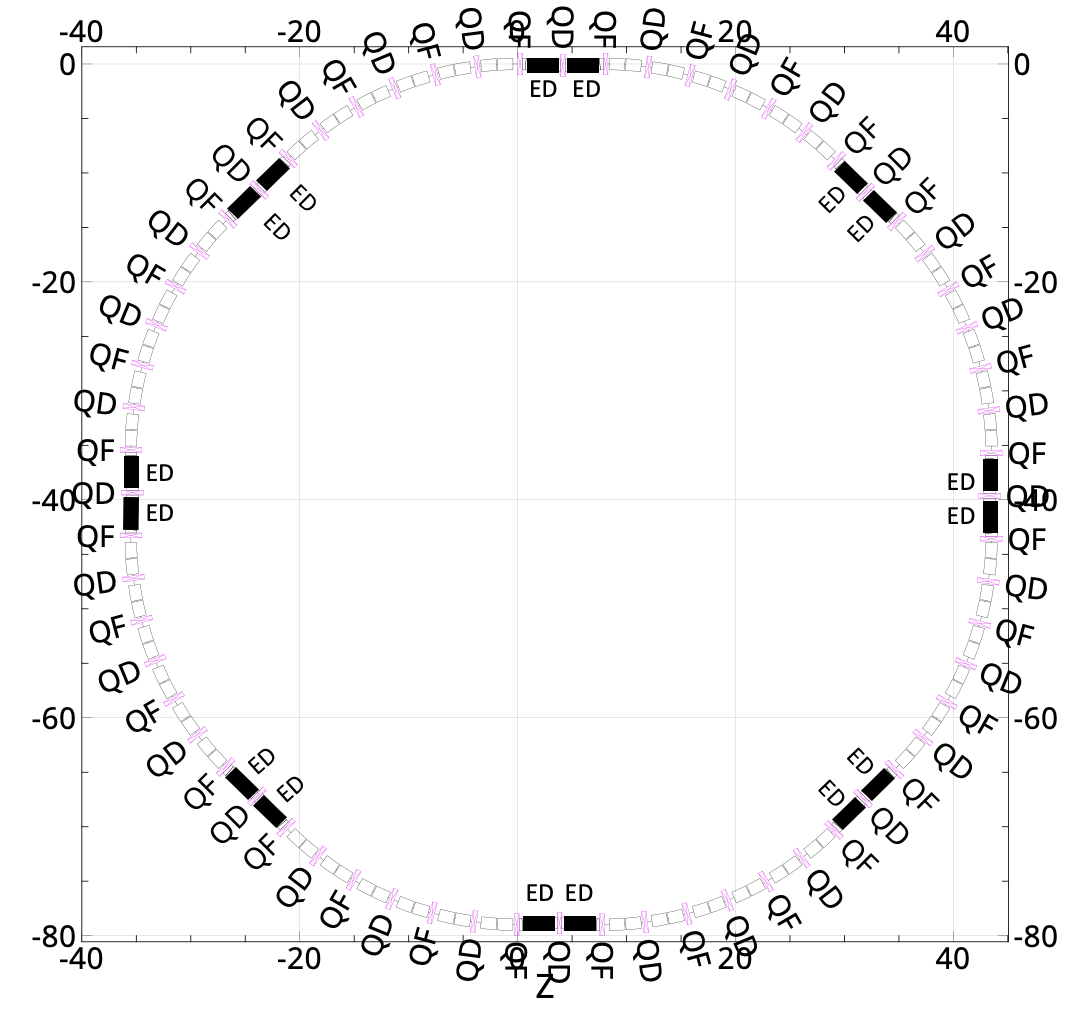
\includegraphics[width=\linewidth]{TEXPaper/img/TUPS031_f3}};
			\end{tikzpicture}
			\centering Current lattice w deflectors
		\end{minipage}
		\hfill
		\begin{minipage}{0.34\linewidth}
			\begin{tikzpicture}
			\node (cone) at (0,0) {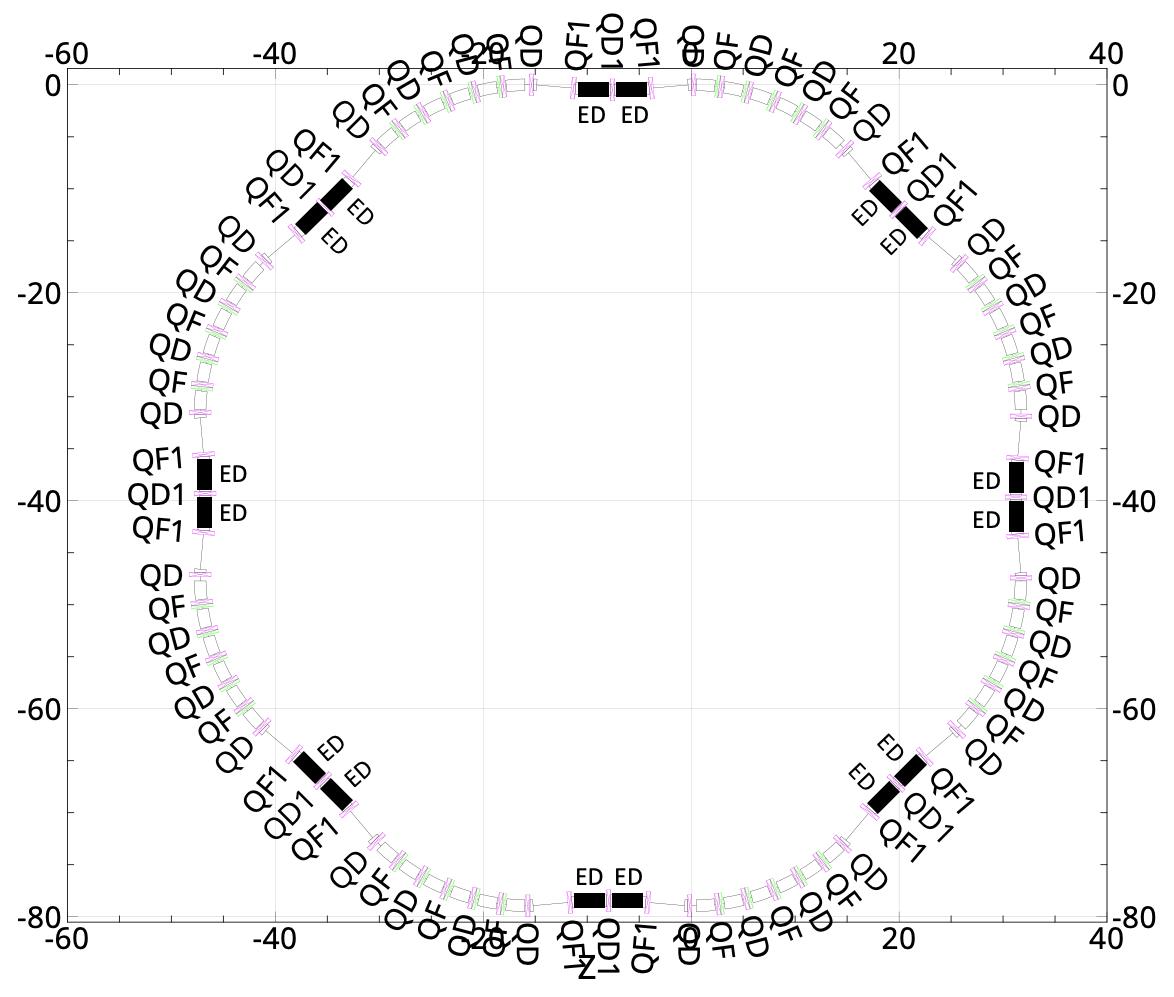
\includegraphics[width=\linewidth]{TEXPaper/img/TUPS031_f4}};
			\end{tikzpicture}
			\centering Modernization I
		\end{minipage}
		\hfill
		\begin{minipage}{0.34\linewidth}
			\begin{tikzpicture}
			\node (cone) at (0,0) {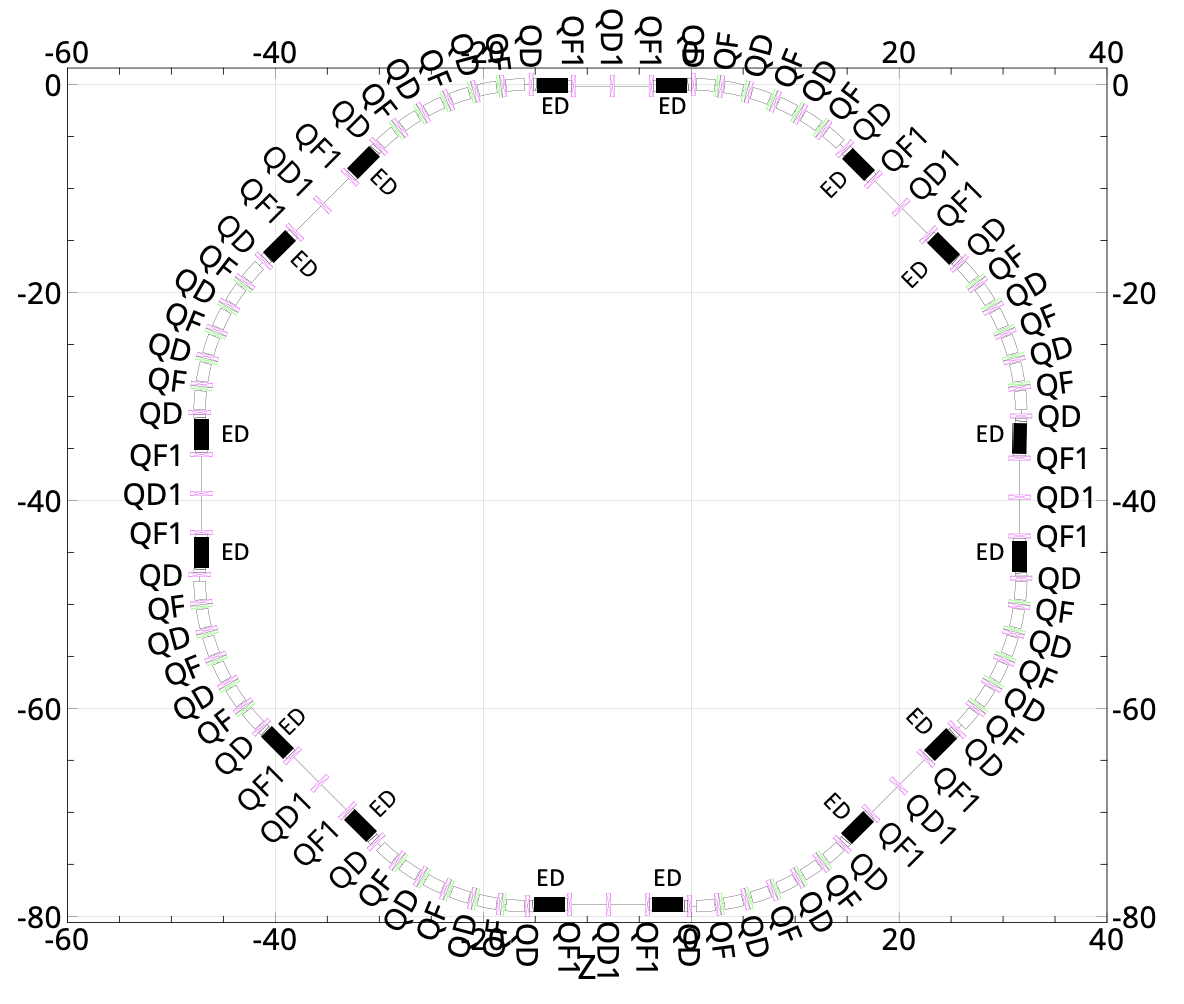
\includegraphics[width=\linewidth]{TEXPaper/img/TUPS031_f5}};
			\end{tikzpicture}
			\centering Modernization II
		\end{minipage}
		\newline \newline
		
		\begin{minipage}{0.49\linewidth}
			\par A primary advantage of the QFS lattice is its capacity to preserve particle acceleration at higher energy levels. The current Nuclotron structure is considered as a NICA collider booster and setup for fixed target experiments. For electric field $E=13$ MV/m the total deflector length $L_{\text{el}}=53$ m for deuterons. The maximum distance is 17 cm between two beampipes: pure straight section and bypass. It is not enough to locate both necessary equipment at straight section and deflector at bypass.
		\end{minipage}
		\hfill
		\begin{minipage}{0.49\linewidth}
		\par Modernized Nuclotron lattice is considered in order to make longer straight sections and install equipments consistently and not to overlap each other. This require to make dipole magnets shorter, here considered the transition from 1.44 to 1.8 T and total magnet length changes from 200 to 150 m accordingly. There are two ways how electrostatic deflectors can be implemented: 1) at the centre; 2) at the edges. The maximum distance between two beampipes are $47$ cm and $50$ cm, respectively.
		\end{minipage}
		
}

	\block{CONCLUSION}{
	\begin{minipage}{0.49\linewidth}
			\par The implementation of a quasi-frozen spin structure presents a periodic lattice with electrostatic deflector to study the EDM of charged particle. The design achieves precise spin compensation of MDM-effect by employing elements with matched curvatures for electric and magnetic fields.
	\end{minipage}
	\hfill
	\begin{minipage}{0.49\linewidth}
		\par Considered the current Nuclotron structure and a possible QFS modernization with a high magnetic field in dipoles. The study demonstrates the versatility of the quasi-frozen spin lattice, which can be adapted for multiple purposes, including higher-energy research within existing facilities.
	\end{minipage}
}

	\block{REFERENCES}{\hfill
	
	\par [1] V.Bargmann, L.Michel, V.L.Telegdi, Precession of the Polarization of Particles Moving in a Homogeneous Electromagnetic Field. Phys. Rev. Lett. \textbf{2}, 435 (1959). doi:10.1103/PhysRevLett.2.435
	\par [2] V.Anastassopoulos et al., A Storage Ring Experiment to Detect a Proton Electric Dipole Moment. Rev.Sci.Instrum. \textbf{87}, 115116 (2016). doi:10.1063/1.4967465
	\par [3] Yu.Senichev et al., in \textit{ICAP2015 Proccedings}, Shanghai, 2016, ed. by C.Kwok, R.W.Volker, T.Chuanxiang, Y.Heping
	\par [4] A.Aggarwal, A.Magiera, Controlling Systematic Uncertainties in Search for an EDM in the Storage Ring. Acta Phys. Pol. B \textbf{51}, 373 (2020) doi:10.5506/APhysPolB.51.373
	\par [5] M.W.Mcnaughton el al., THE P C ANALYZING POWER BETWEEN 100-MEV AND 750-MEV. Nuc. Inst. and Meth. in Phys. Res. Sec. A \textbf{241}, 435-440 (1985). doi:10.1016/0168-9002(85)90595-9
	}
	
\end{columns}

\end{document}